\section{Training Algorithm}

% mention the best_model during collect_rollouts
% mention this is because the real full eval is expensive


The neural network training process consists of a simple training loop. In each iteration, the algorithm collects data from the environment. The data is stored in a replay buffer. After collecting the data, the model is trained on the data in the replay buffer. The training process is repeated until a certain number of timesteps has been collected.  

In most reinforcement learning algorithms, the trained model's performance is evaluated at short intervals. The frequent evaluations serve as a way to monitor the model's performance during training and measure progress. It is not guaranteed in reinforcement learning that a model improves during each model update. Therefore frequent evaluations also help in finding the best version of the model.  
In this training algorithm there is no dedicated evaluation process at short intervals. Instead the episodes from the data collection step are used to evaluate the model at every iteration of the training loop. This saves computational resources compared to a full evaluation of the model.

\renewcommand{\thepseudonum}{\roman{pseudonum}}
\begin{pseudocode}{TrainNetwork}{ }
\label{train_network}
\COMMENT{Main Training Algorithm}\\

\MAIN
Env \GETS \CALL{Environment}{environment\_parameters}\\
RolloutBuffer \GETS \CALL{RolloutBuffer}{rollout\_buffer\_size}\\
Model \GETS \CALL{Model}{model\_parameters}\\
Optimizer \GETS \CALL{Optimizer}{optimizer\_parameters}\\

num\_timesteps \GETS 0\\
\WHILE num\_timesteps < total\_timesteps \DO 
\BEGIN 
num\_collected\_steps \GETS \CALL{CollectData}{}\\
num\_timesteps \GETS num\_timesteps + num\_collected\_steps\\
\CALL{TrainModel}{}\\
\END\\
\ENDMAIN
\end{pseudocode}

\subsection{Collect Data}

The data is stored in a replay buffer for use by the training algorithm. The data collection process starts by resetting the replay buffer, this removes the collected sampled of previous iterations from memory.
The data collection process is a simple loop that collects a fixed amount of samples from the environment. The reinforcement learning algorithm Proximal Policy Optimization requires that the samples are collected on-policy. As a result the most recently updated model is used to chose actions during the data collection. 

The data collection algorithm starts a new episode and applies the policy to the environment until the episode terminates. The observation is used to prompt the model for an action. The action is then applied to the environment, resulting in a reward and a new environment state. The observation, action and reward tuples are stored in the replay buffer. A new episode is started upon termination of the current episode. The data collection process continues until the replay buffer is full.

\paragraph{Environment settings for Data collection}

The environment settings define how the episodes are reset during the data collection process. The episodes are initialized according to the parameters trainingMapType, trainingLightSetting and spawnOrientation \ref{fig:env_reset_settings}. The settings influence the difficulty and variety of the tracks. The settings define what data the agent policy can learn from during training.

Different configurations are used in the experimentation phase to gain insights into the network's capabilities.


\begin{figure}
    
    \begin{center}
    \begin{tabular}{|| c | p{0.25\linewidth} | p{0.4\linewidth} ||} 
        \hline
        Parameter name & Options & Explanation  \\ [0.5ex] 
        \hline\hline
        \multirow{4}{*}{trainingMapType} & randomEvalEasy & Selects a random easy track. \\\cline{2-3}
        & randomEvalMedium & Selects a random medium track. \\\cline{2-3}
        & randomEvalHard & Selects a random hard track. \\\cline{2-3}
        & randomEval & Selects a random track from all difficulties. 20\% easy, 40\% medium, 40\% hard \\
        \hline
        \multirow{4}{*}{trainingLightSetting} & bright & Bright illumination. \\\cline{2-3}
        & standard & Standard illumination. \\\cline{2-3}
        & dark & Dark illumination. \\\cline{2-3}
        & random & Selects a random light setting from bright, standard and dark. \\
        \hline
        \multirow{4}{*}{spawnOrientation} & Fixed & Spawn JetBot with fixed coordinates and orientation. \\\cline{2-3}
        & Random & Spawn JetBot with fixed coordinates and random orientation (-15 to 15 degrees). \\\cline{2-3}
        & VeryRandom & Spawn JetBot with fixed coordinates and random orientation (-45 to 45 degrees). \\
        \hline
    \end{tabular}
    \end{center}
    \caption{Environment parameters for training.} % the parameters are already defined in endDescription
    \label{fig:env_reset_settings}
\end{figure}

\paragraph{Evaluation of the model}

There is no dedicated evaluation step in this training algorithm. The collected episodes are analysed to gain insight into the policy's performance during training. No episodes are executed solely for the purpose of measuring the policy's performance during training. The full evaluation of the model as described in \ref{sec:basic_evaluation_algorithm} is time-consuming. The full evaluation process is only executed after the training process has finished, this speeds up training tremendously.

The collected episodes are used to evaluate the model during training. The success rate of the collected episodes is used to determine the best model. The model is saved to disk if the success rate of the collected episodes improved.


The success\_rate and other statistics about the collected episodes are logged to tensorboard to monitor the training process. Example metrics are the goal\_completion\_rate and the collected weighted rewards.
These metrics can show how the policy behaves over time. They show if the policy is able to learn from the collected episodes \ref{fig:metrics_over_time}.

\begin{figure}
    \centering
    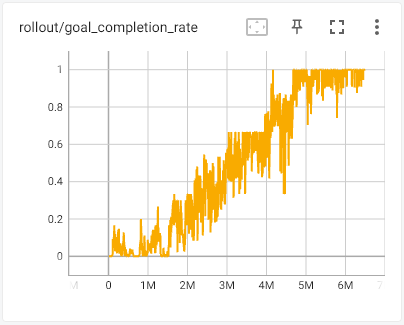
\includegraphics[width=0.4\textwidth]{Bilder/tensorboard_images/successfulTraining_goal_completion_rate.png}
    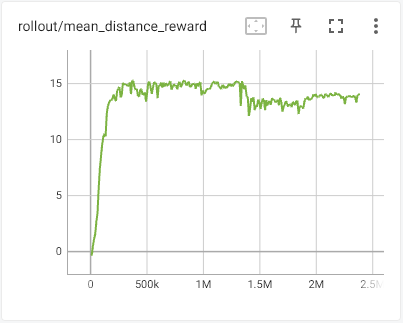
\includegraphics[width=0.4\textwidth]{Bilder/tensorboard_images/successfulTraining_distance_reward.png}
    \caption{Metrics from collected episodes during a successful training}
    \label{fig:metrics_over_time}
\end{figure}


\subsection{Train Model}

The model training part of the algorithm is very conventional and follows the standard implementation of PPO training. The model is trained on the collected data for a fixed number of epochs. In each epoch the replay buffer is sampled to create batches of data. The loss is computed for each batch. The gradient of the weights with respect to the loss is computed using backpropagation. The optimizer is then used to update the model parameters using the gradients.

The entire data from the replay buffer is sampled in every epoch. This ensure that the collected data is used efficiently. The data is shuffled before creating the batches. This ensures that the samples are less correlated and the model updates are more stable.
% the ppo paper uses gradient ascent

\subsubsection*{Loss function}

The loss function follows the Proximal Policy Optimization algorithm \textcite{ppo}. The PPO loss function is a combination of the policy surrogate and value error. The policy surrogate and value error are combined to be able to update the weights of the entire neural network together.

The policy surrogate objective function is responsible for improving the policy's output action distribution. The function behaves similarly to other policy update based aproaches. It restricts the size of parameter updates, increasing the stability during training. The ratio between the old and the current policy is clipped. The clipped ratio and non-clipped ratio are multiplied by the advantage. The minimum of the two is used as the policy surrogate loss. This prevents the updates from changing the policy drastically.

The advantage is an estimator for how much better (or worse) the policy performed than expected. The advantage $\hat{A}_t$ is computed using the value estimates produced by the neural network. The multiplication of the ratio with the advantage leads to increased probabilities for good actions and decreased probabilities for bad actions.

The value error is responsible for improving the policy's output value estimates. The value error is the mean squared error between the predicted value and the target value. The parameter changes caused by the value error lead to a more accurate value prediction.

The policy loss can also include an entropy term. Similarly to the original paper \textcite{ppo}, no entropy term is used in this work. This results in the loss function \eqref{eq:eq1} with the value coefficient $c_1 = 0.5$.

\begin{align*}
    L_t^{CLIP + VF} &= \hat{\mathbb{E}}_t [L_t^{CLIP}(\theta) - c_1 L_t^{VF}(\theta)] \label{eq:eq1}\tag{PPO Loss} \\
    L_t^{CLIP}(\theta) &= min(r_t(\theta)\hat{A}_t, clip(r_t(\theta), 1-\epsilon, 1+\epsilon)\hat{A}_t) \label{eq:eq2}\tag{Surrogate Objective}\\
    r_t(\theta) &= \frac{\pi_\theta(a_t|s_t)}{\pi_{\theta_{old}}(a_t|s_t)} \label{eq:eq3}\tag{Ratio}\\
    L_t^{VF}(\theta) &= (V_\theta (s_t) - V_t^{targ})^2 \label{eq:eq4}\tag{Value Error}
\end{align*}
% for the target value + advantage computation see my_buffers.compute_returns_and_advantage returns

\subsection{Final Result of Training Algorithm}

Weight updates can lead to a decrease in performance during the training process. The model after the final weight update is not guaranteed to be the best observed version.
The model performance is evaluated during training using the collected episodes. The model with the highest observed success\_rate is considered to be the final output of the training algorithm. This model is later used for the full evaluations.

